\documentclass[a4paper,10pt]{article}
\usepackage[utf8]{inputenc}

% ----  Useful packages % ---- 
\usepackage{amsmath}
\usepackage{graphicx}
\usepackage{amsfonts}
\usepackage{amsthm}
\usepackage{amssymb}
\usepackage{makecell}
\usepackage{array}
\usepackage{booktabs}
\usepackage{multirow}
\usepackage{wrapfig}
\usepackage{subfigure}
\usepackage{enumitem}
% ----  Useful packages % ---- 

\usepackage{wrapfig}
\usepackage{caption}
\usepackage{subcaption}
\usepackage{hyperref}
\hypersetup{
    colorlinks,
    citecolor=black,
    filecolor=black,
    linkcolor=black,
    urlcolor=black
}
\usepackage{wrapfig}

\graphicspath{ {./images/} }

\setcounter{tocdepth}{6}

% ---- Set page size and margins replace ------
\usepackage[letterpaper,top=2cm,bottom=2cm,left=3cm,right=3cm,marginparwidth=1.75cm]{geometry}
% ---- Set page size and margins replace ------

% ------- NOTA ------
\theoremstyle{remark}
\newtheorem{note}{Note}[subsubsection]
% ------- NOTA ------

% ------- OSSERVAZIONE ------
\theoremstyle{definition}
\newtheorem{observation}{Observation}[subsection]
% ------- OSSERVAZIONE ------

% ------- DEFINIZIONE ------
\theoremstyle{plain}
\newtheorem{definition}{Definition}[subsection]
% ------- DEFINIZIONE ------

% ------- ESEMPIO ------
\theoremstyle{definition}
\newtheorem{example}{Example}[subsection]
% ------- ESEMPIO ------

% ------- DIMOSTRAZIONE ------
\theoremstyle{definition}
\newtheorem{question}{Question}[subsection]
% ------- DIMOSTRAZIONE ------

% ------- TEOREMA ------
\theoremstyle{definition}
\newtheorem{theorem}{Theorem}[subsection]
% ------- TEOREMA ------

% ------- COROLLARIO ------
\theoremstyle{plain}
\newtheorem{corollaries}{Corollario}[theorem]
% ------- COROLLARIO ------

% ------- PROPOSIZIONE ------
\theoremstyle{plain}
\newtheorem{proposition}{Proposizione}[subsection]
% ------- PROPOSIZIONE ------

% ---- Footer and header ---- 
\usepackage{fancyhdr}
\pagestyle{fancy}
\fancyhf{}
\fancyhead[LE,RO]{WS 2024/2025}
\fancyhead[RE,LO]{Computer Architecture}
\fancyfoot[RE,LO]{\rightmark}
\fancyfoot[LE,RO]{\thepage}

\renewcommand{\headrulewidth}{.5pt}
\renewcommand{\footrulewidth}{.5pt}
% ---- Footer and header ---- 

% ----  Language setting ---- 
\usepackage[italian, english]{babel}
% ----  Language setting ---- 

\usepackage{listings}
\usepackage{color}

\definecolor{dkgreen}{rgb}{0,0.6,0}
\definecolor{gray}{rgb}{0.5,0.5,0.5}
\definecolor{mauve}{rgb}{0.58,0,0.82}

\lstset{frame=tb,
  language=C,
  aboveskip=3mm,
  belowskip=3mm,
  showstringspaces=false,
  columns=flexible,
  basicstyle={\small\ttfamily},
  numbers=none,
  numberstyle=\tiny\color{gray},
  keywordstyle=\color{blue},
  commentstyle=\color{dkgreen},
  stringstyle=\color{mauve},
  breaklines=true,
  breakatwhitespace=true,
  tabsize=3
}

\title{\textbf{Computer Architecture}}
\author{Autor: Ghirardini Filippo}
\date{Winter Semester 2024-2025}

\begin{document}
\begin{titlepage} %crea l'enviroment
	\begin{figure}[t] %inserisce le figure
		\centering
\includegraphics[width=0.98\textwidth]{marchio_unipi_pant541.png}
	\end{figure}
	\vspace{20mm}
	
	\begin{Large}
		\begin{center}
			\textbf{Dipartimento di Informatica\\ Corso di Laurea Triennale in Informatica\\}
			\vspace{20mm}
			{\LARGE{Corso a Libera Scelta - 6 CFU}}\\
			\vspace{10mm}
			{\huge{\bf Computer Graphics}}\\
		\end{center}
	\end{Large}
	
	
	\vspace{36mm}
	%minipage divide la pagina in due sezioni settabili
	\begin{minipage}[t]{0.47\textwidth}
		{\large{\bf Professore:}\\ \large{Prof. }}
	\end{minipage}
	\hfill
	\begin{minipage}[t]{0.47\textwidth}\raggedleft
		{\large{\bf Autore:}\\ \large{Filippo Ghirardini}}
	\end{minipage}
	
	\vspace{25mm}
	
	\hrulefill
	
	\vspace{5mm}
	
	\centering{\large{\bf Anno Accademico 2023/2024 }}
	
\end{titlepage}

\tableofcontents
\newpage
\maketitle
\begin{center}
    \vspace{-20pt}
    \rule{11cm}{.1pt} 
\end{center}
\newpage
\section{Punto materiale}
Oggetto caratterizzato da una massa [kg] e da un vettore posizione [m] nello spazio 3D.
Dimensioni trascurabili, forma irrilevante rispetto ai fenomeni di interesse.
Vettore posizione come funzione del tempo t[s].
\begin{example}
    Una molecola di ossigeno se sono interessato all'aereodinamica di una vettua. 
    Un satellite attorno alla terra se ignoro le forze di marea.
\end{example}
\hspace{-15pt}\textbf{Un vettore posizione} è una funzione del tempo $t[s]$.
$$\vec{r(t)} = (x(t), y(t), z(t)) = x(t)\hat{x} + y(t)\hat{z} + z(t)\hat{z}$$
\begin{observation}
    I versori cartesiani sono costanti
\end{observation}

\begin{definition}[Legge oraria]
    Si definisce come legge oraria la funzione $t \mapsto \vec{r}(t)$.
\end{definition}

\begin{definition}[Traiettoria]
    Il luogo geometrico di punti visitati dal punto materiale.
    $$\{\vec{r}(t)\:\: per \: t \in \mathbb{R}\}$$
\end{definition}

\begin{example}
    $\vec{r}(t) = (v_0t, y_0, 0)$ e $v_0 = 3m/s, y_o = 5m$ 
    \begin{figure}[h!]
        \centering
        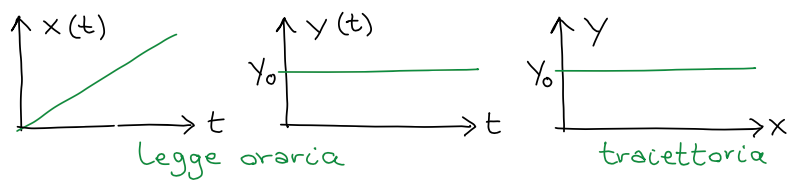
\includegraphics[width=0.8\textwidth]{images/ess-traiettoria.png}
    \end{figure}
\end{example}

\begin{definition}
    La \textbf{velocità istantanea} è la derivata della posizione rispetto al tempo.
    $$v = \lim_{\Delta t \to 0}\frac{\Delta s}{\Delta t} = \frac{ds}{dt}$$
\end{definition}

\begin{definition}
    La \textbf{velocità media} è definita come il rapporto tra lo spostamento e l'intervallo di tempo necessario per effettuarlo.
    $$v_m = \frac{\Delta s}{\Delta t}$$
\end{definition}
\hspace{-15pt}In parole povere è una grandezza che ci dice con quale rapidità cambia la posizione di un punto rispetto al tempo nell'instante $t$.
\subsection*{Vettore velocità}
Derivata rispetto al tempo del vettore posizione e si indica come 
$\frac{d\vec{r}(t)}{dt}\text{ oppure }\dot{\vec{r}}(t)[m/s]$
\begin{equation}
    \begin{split}
    \dot{\vec{r}}(t) & = (\dot{x}(t), \dot{y}(t), \dot{z}(t)) \\
     & = \frac{d}{dt}[x(t)\hat{x} + y(t)\hat{y} + z(t)\hat{z}] \\
     & = \dot{x}(t)\hat{x} + \dot{y}(t)\hat{y} + \dot{z}(t)\hat{z}
    \end{split}
\end{equation}
Per ricavare la forma esplicita uso le proprietà delle derivate (\textbf{linearità}, \textbf{Leibnitz})
\begin{example}
    $\vec{r}(t) = (v_0t, y_0, 0) = v_0t\hat{x} + y_0\hat{y}$ \:\:\:abbiamo che \:\:\:
    $\dot{\vec{r}}(t) = (v_0, 0, 0) = v_0 \hat{x}$
\end{example}
\hspace{-15pt}Velocità e spazio percorso ("integrale di linea").\\
\begin{wrapfigure}[3]{l}{5cm}
    \centering
    \includegraphics[width=5cm]{images/vettore-velocità.png}
\end{wrapfigure}
\begin{align*}
    L & = ||\vec{r}(t_1) - \vec{r}(t_0)|| + ||\vec{r}(t_2) - \vec{r}(t_1)|| + ||\vec{r}(t_3) - \vec{r}(t_2)|| + \dots \\
    & = \sum_i ||\vec{r}(t_{i+1} - \vec{r}(t_i)|| \:\: per\:\: |t_{i+1} - t_i| \text{"piccolo"} \\
    & = \sum_i ||\frac{\vec{r}(t_{i+1}) - \vec{r}(t_i)}{t_{i+1} - t_i}|| (t_{i+1} - t_i) = \int_{t_{in}}^{t_{f_{in}}}||\dot{\vec{r}}(t)||\\
\end{align*}
\begin{example}
    $\vec{r}(t) = (v_0t, y_0)\:\:\: \dot{\vec{r}}(t) = (v_0, 0)$\hspace{15pt}
    $||\dot{\vec{r}}(t)|| = \sqrt{v_0^2 + 0^2} = |v_0|$ \:\:\: $L = |v_0| \cdot (t_{f_{in}} - t_{in})$\\
    Il vettore è costante quindi facendo la derivata torna zero. Con la velocità si calcolo lo spazio percorso ("integrale di linea").
    La differenza fra le posizioni e la differenza dei tempi è il rapporto incrementale in caso gli intervalli siano sufficentemente
    piccoli, da qui si ottiene l'integrale.
\end{example}

\subsection{Vettore accelerazione}
Derivata rispetto al tempo del vettore velocità e si indica con $\frac{d^2\vec{r}(t)}{dt} \text{ oppure } \ddot{\vec{r}}(t) [m/s^2]$
\begin{equation}
    \ddot{\vec{r}}(t) = (\ddot{x}(t), \ddot{y}(t), \ddot{z}(t))\:\: = \:\: \ddot{x}(t)\hat{x} + \ddot{y}(t)\hat{y} + \ddot{z}(t)\hat{z}
\end{equation}
\begin{example}
    $\vec{r}(t)= (\frac{1}{2}a_0t^2, v_0t, 0)$ \hspace{10pt} $\dot{\vec{r}}(t) = (a_0t, v_0, 0)$ \hspace{10pt} $\dot{\vec{r}}(t) = (a_0, 0, 0)$
\end{example}
\hspace{-15pt}Serve perché l'equazione "del moto" di Newton che determinata la legge oraria è formulata in termini di accelerazione.

\subsection{Vettore quantità di moto}
Il prodotto di massa [kg] e velocità [m/s]
$$\vec{p}(t) = m \cdot \dot{\vec{r}}(t) = (m\dot{x}(t), m\dot{y}(t), m\dot{x}(t)) = m\dot{\vec{x}}(t)x + m\dot{\vec{y}}(t)y + m \dot{\vec{z}}(t)z$$
\begin{example}
    Prendiamo un punto di massa 2kg e velocità 3m/s lungo $\hat{x}$.\\
    $p_x(t) = 2 \cdot 3 kg\cdot m/s = 6 kg \cdot m/s$ \hspace{15pt} $p_y(t) = p_z(t) = 0$.
\end{example}
\hspace{-15pt}Serve per generalizzare l'equazione di Newton e per trattare sistemi di piu punti materiali.

\subsection{Vettore momento angolare rispetto a un polo P}
$$\vec{L}_p(t) = m(\vec{r}(t) - \vec{r}_p) \times \dot{\vec{r}}(t)$$
Dove $\vec{r}_p$ è il vettore posizione di p, mentre $\dot{\vec{r}}(t)$ è il prodotto vettoriale.
\begin{example}
    $\vec{r}_p = (l_0, 0, 0)$ \hspace{15pt} $\vec{r}(t) = (v_0t, y_0, 0)$\\
    $\vec{L}_p = m[(v_0t - l_0)\hat{x} + y_0\hat{y}] \times (v_0\hat{x}) \:\: = \:\: m(v_0t - l_0)v_0 \hat{x} \times \hat{x} + my_0v_0\hat{y}\times \hat{x} 
    \:\: = \:\: my_0v_0(-\hat{z}) = (0,0, -my_0v_0)$\\
    Ricorda che $\hat{x} \times \hat{x} = 0$ e $\hat{y} \times \hat{x} = -\hat{z}$
\end{example}
\hspace{-15pt}Il momento angolare dice quanta inerzia ha un oggetto in una rotazione (descrizione sommaria).\\
Il polo P è parte della definizione. È una scelta! Il risultato dipende dal polo.
Serve per formulare l'equazione del moto di sistemi di punti materiali e corpi rigidi.

\subsection{Coordinate polari}
Un metodo per rapprensentare delle cordinate x, y andando a misurare prima la distanza dall'origine e poi si va a vedere
quanto vale l'angolo fra questo segmento dall'asse x, utilizzando seno e coseno.
\begin{wrapfigure}[7]{l}{2cm}
    \centering
    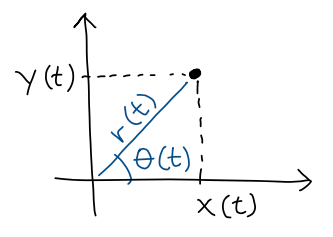
\includegraphics[width=5.5cm]{images/coordinate-polari.png}
\end{wrapfigure}
\begin{align*}
    \begin{cases}
        x(t) = r(t) \cdot \cos(\Theta(t))\\
        y(t) = r(t) \cdot \sin(\Theta(t)) 
    \end{cases}
\end{align*}
\begin{align*}
    \begin{cases}
        r(t) = \sqrt{x(t)^2 + y(t)^2} \geq 0\\
        tg(\Theta(t)) = y(t) / x(t) 
    \end{cases}
\end{align*}
\\
\begin{example} Esempi di rappresentazione di coordinate in coordinate polari.\\
    $x = 0, y = l_0 > 0 \:\: \Rightarrow \:\: r = l_0, \Theta = \pi/2$\\
    $x = 0, y = -l_0 < 0 \:\: \Rightarrow \:\: r = l_0, \Theta = -\pi/2$\\
    $x = l_0, y = l_0 > 0 \:\: \Rightarrow \:\: r = \sqrt{2}l_0, \Theta = \pi/4$\\
\end{example}

\subsection{Versori polari (2D)}
Definisco un versore $\hat{r}(t)$ che punta verso il punto materiale e un versore $\hat{\Theta}(t)$ ortogonale.
Si esprime facilmente in coordinte polari.
$$\vec{r}(t) = (x(t), y(t)) = (r(t)\cos \Theta(t), r(t)\sin\Theta(t)) \:\: = \:\: r(t)(\cos\Theta(t)\hat{x} + \sin\Theta(t)\hat{y})$$
Ma $||\vec{r}(t)|| = |r(t)| = r(t)$ allora definisco $\hat{r}(t) = \vec{r}(t)/ ||\vec{r}(t)|| = \cos \Theta(t)\hat{x} + \sin\Theta(t)\hat{y}$\\\\
Trovo facilmente che un versore ortogonale è:
$$\hat{\Theta(t)} = -\sin\Theta(t)\hat{x} + \cos\Theta(t)\hat{y} \:\:\:\text{infatti} \:\:\: \hat{r}\cdot \hat{\Theta} = c \cdot (-s) + s \cdot c = 0$$
\begin{wrapfigure}[7]{r}{6cm}
    \centering
    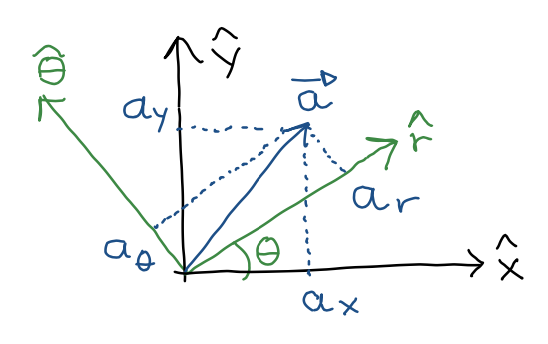
\includegraphics[width=5.5cm]{images/trasformazioni-inverse.png}
\end{wrapfigure}
\begin{note}
    Non c'è legame fra $\Theta$ e $\hat{\Theta}$ è solo una convenzione.
\end{note}
\hspace{-15pt}Le trasformazioni inverse invece si fanno come segue (verifico per sostituzione):
$$\hat{y} = \cos\Theta(t)\hat{r} - \sin\Theta(t)\hat{\Theta} \hspace{20pt} \hat{y} = \sin\Theta(t)\hat{r} + \cos\Theta(t)\hat{\Theta}$$
Possono quindi scrivere ogni vettore nella forma $\vec{a} = a_r\hat{r} + a_{\Theta}\hat{\Theta}$ con le componenti polari $a_r, a_{\Theta}$.
Per evitare ambiguità non scriviamo $(a_r, a_{\Theta})$ e riserviamo la notazione alle componenti cartesiane.\\\\
A differenza dei versori cartesiani quelli polari dipendono dal tempo per costruzioni.
$$\dot{\hat{r}}(t) = \frac{d}{dt}[\cos\Theta(t) \hat{x} + \sin\Theta(t)\hat{y}] \:\: = \:\: -\sin\Theta(t) \cdot \dot{\Theta}(t)\hat{x} + \cos\Theta(t) \cdot \dot{\Theta}(t)\hat{y}$$
Dove $\cos\Theta(t) \cdot \dot{\Theta}(t)$ si applica la derivata della somma, Leibnitz, funzione composta.
$$= \dot{\Theta}(t)\cdot \hat{\Theta}(t) \:\:\:\:(\text{confronto l'espressione di} \hat{\Theta}(t))$$
Similmente $\dot{\hat{\Theta}}(t)= - \dot{\Theta}\hat{r}(t)$.


\subsection*{Vettori posizione, velocità, accelerazione}
$$\vec{r}(t) = r(t)\hat{r}(t)$$
Dove abbiamo che $\vec{r}(t)$ è il vettore, $r(t)$ è una coordinata polare, $\hat{t}(t)$ è il versore polare.
$$\dot{\vec{r}}(r) = \dot{r}(t)\hat{r}(t) + r(t)\dot{\Theta}(t)\hat{\Theta}(t)$$
Dove la parte $\dot{\vec{r}}(r)$ è la velocità radiale.
$$\ddot{\vec{r}}(t) = [\ddot{r}(t) - r(t)\dot{\Theta}(t)^2] \hat{r} + [r(t) \ddot{\Theta}(t) + 2\dot{r}(t)\dot{\Theta}(t)]\hat{\Theta}$$
Nel quale abbiamo che la parte $r(t)\dot{\Theta}(t)^2$ si chiama \textbf{velocità centripeta}, mentre $2\dot{r}(t)\dot{\Theta}(t)$ si dice \textbf{accelerazione di Coriolis}.


% !TeX spellcheck = en_US
\newpage
\section{Data arithmetic}
\subsection{Number systems}
\begin{definition}[Positional]
	Representation of numbers as a sequence of digits $z_i$, with the radix point between $z_0$ and $z_{-1}$:
	\begin{equation}
		-z_n z_{n-1} \ldots z_1 z_0 . z_{-1} z_{-2} \ldots z_{-m}
	\end{equation}
	Each position $i$ of the sequence of digits is assigned a value, which is a power $b_i$ of the base $b$ of the numbering system:
	\begin{equation}
		X_b = z_n\cdot b ^n + z_{n-1} \cdot b^{n-1} + \ldots + z_1 \cdot b^1 + z_0 \cdot b^0 + z_{-1} \cdot b^{-1} + \ldots + z_{-m} \cdot b^{-m} = \sum_{i=-m}^{n} z_i \cdot b^i\label{eq:1}
	\end{equation}
\end{definition}

Common bases of numbering systems used in computer science are:
\begin{table}[!h]
	\centering
	\begin{tabular}{|c|c|c|}
		\hline
		 \textbf{Base (b)} & \textbf{Number system} & \textbf{Alphabet} \\
		 \hline
		 $2$ & Binary & $0, 1$ \\
		\hline
		$8$ & Octal & $0,1,2,3,4,5,6,7$ \\
		\hline
		$10$ & Decimal & $0,1,2,3,4,5,6,7,8,9$ \\
		\hline
		$16$ & Hexadecimal & $0,1,2,3,4,5,6,7,8,9,A,B,C,D,E,F$ \\
		\hline
	\end{tabular}
\end{table}

\subsection{Conversion FROM decimal}
\subsubsection{Euclid}
Considering the following representation of a number that we want to convert in a base $b$:
\begin{align*}
	& Z = z_n\cdot 10^n + z_{n-1} \cdot 10^{n-1} + \ldots + z_1 \cdot 10 + z_0 + z_{-1} \cdot 10^{-1} + \ldots + z_{-m} \cdot 10^{-m} = \\
	& = y_p\cdot b ^p + y_{p-1} \cdot b^{p-1} + \ldots + y_1 \cdot b+ z_0 + y_{-1} \cdot b^{-1} + \ldots + y_{-q} \cdot b^{-q}
\end{align*}
we generate the digits step by step starting with the most significant (leftmost):
\begin{enumerate}
	\item Search $p$ according to the inequation
	\begin{equation*}
		b^p \leq Z < b^{p+1}
	\end{equation*}
	and assign $i=p$ and $Z_i = Z$
	\item Derive $y_i$ and the reminder $R_i$ by division of $z_i$ by $b^i$
	\item Repeat step 2 for $i=p-1, \ldots$ and replace each step $Z_i$ with $R_i$ until $R_i = 0$ or $b^i$ is small enough that the precision is enough
\end{enumerate}
\subsubsection{Horner}
This method is structured in two phases:
\begin{enumerate}
	\item \textbf{Integer} part: factoring out the integer we get
	\begin{equation*}
		X_b = \sum_{i=0}^{n} z_i \cdot b^i = ((\ldots (((z_n \cdot b + z_{n-1}) \cdot b + z_{n-2}) \cdot b + z_{n-3}) \cdot b \ldots) \cdot b + z_1) \cdot b + z_0
	\end{equation*}
	\item \textbf{Decimal} part: we multiply the decimals of the number by base b to get the fractional digits $y_{-i}$ from the most to the least significant position
	\begin{equation*}
		Y_b = \sum_{i=-m}^{-1} y_i \cdot b^i = ((\ldots (((y_{-m} \cdot b^{-1} + y_{-m+1}) \cdot b^{-1} + y_{-m+2}) \cdot b^{-1} + y_{-m+3}) \cdot b^{-1} \ldots) \cdot b^{-1} + y_{-1}) \cdot b^{-1}
	\end{equation*}
\end{enumerate}
\subsection{Conversion TO decimal}
We represent the values of the single positions of the number we want to convert in our common decimal system and sum all values.\\
The value $X_b$ of the number is the sum of all single values of all positions $z_i\cdot b^i$, like in equation \eqref{eq:1}.

\subsection{General conversion}
If we want to convert from an arbitrary system to another, we first convert to decimal and then we use one of the other two methods.

\begin{observation}
	If the base of one system is a power of the base of another system the conversion is done by Replacing a sequence of digits by a single digit or replace a digit by $a$ sequence of digits, respectively.
\end{observation}
% !TeX spellcheck = en_US
\newpage
\section{Microarchitecture}
This section describes level no. 1 from the 6 level model that we saw in \ref{img:levels}.
\subsection{Architecture of a microprocessor}
The internal architecture of a simple microprocessor is designed as follows:
\begin{center}
	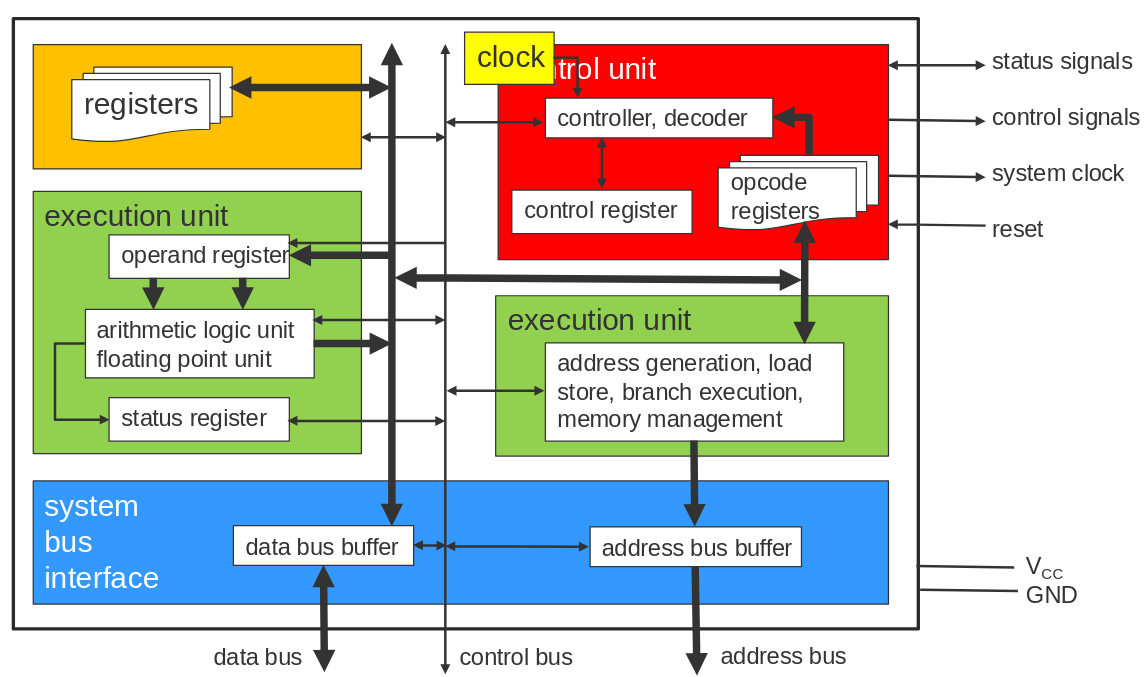
\includegraphics[scale=0.35]{microarchitecture}
\end{center}

\subsubsection{Control unit}

\begin{wrapfigure}[4]{r}{6cm}
	\vspace{-1.1cm}
	\begin{center}
		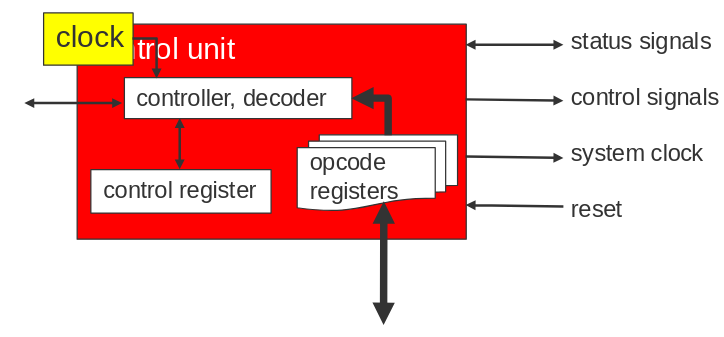
\includegraphics[width=6cm]{controlunit}
	\end{center}
\end{wrapfigure}

The control unit is the part that \textbf{controls} all the other components.
\paragraph{Clock} Generates the system clock for distribution to all components.

\paragraph{Decoder} 
It generates all control signals for the components and uses status signals and opcode as an input. Often \textbf{micro-programmable}.

\begin{definition}[Micro programmable]
	The processor stores a \textbf{microprogram} for each instruction that can be modified only by the manufacturer. Single bits of a \textbf{micro instruction} represents \textbf{micro operations}, thus a setting of the control signals for the components.\\
	Pure \textbf{RISC} processors typically use a fixed sequential circuit instead.
\end{definition}

\noindent The \textbf{phases of execution} of an instruction is composed of:
\begin{enumerate}
	\item \textbf{Fetch}: load the next instruction into the opcode register
	\item \textbf{Decode}: get the start address of the microprogram representing the instruction
	\item \textbf{Execute}: the microprogram controls the instruction execution by sending the appropriate signals to the other components and evaluating the returned signals
\end{enumerate}

\paragraph{Opcode register}
It contains the portion of the \textbf{instruction} that specifies the currently executed operation to be performed and eventual \textbf{opcodes}. It has \textbf{several registers} because:
\begin{itemize}
	\item Different instructions may have \textbf{different sizes}
	\item Opcode \textbf{prefetching} may speed up program execution: while decoding the current instruction the following one may be prefetched
\end{itemize}

\paragraph{Control register}
It stores the current status of the control unit. The meaning of the different bits depend on the specific processor. Some examples:
\begin{itemize}
	\item \textit{Interrupts} enable: determines if the processor reacts to interrupts
	\item \textit{VM extension} enable: enable HW assisted virtualization on x86 CPUs
	\item \textit{User mode instruction prevention}: if set, certain instructions cannot be executed in user level
\end{itemize}

\subsubsection{Execution unit}
\begin{wrapfigure}[8]{r}{5cm}
	\vspace{-0.5cm}
	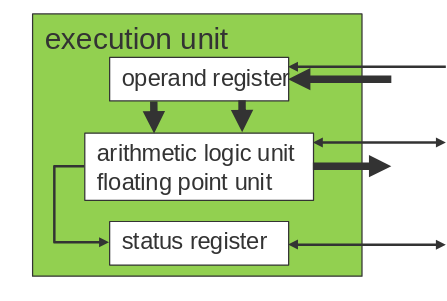
\includegraphics[width=5cm]{execunit1}
\end{wrapfigure}
The execution unit executes all \textbf{logic} and \textbf{arithmetic operations} controlled by the control unit (e.g. int and float arithmetic, logic operations, address operations).

\paragraph{Communication with control unit}
Single bits of a micro instruction directly control the ALU operation and its operands.
\begin{example}
	Example of micro instruction that sets $S_3$, $S_4$ and $S_5$:
	\begin{center}
		\begin{table}[!h]
			\centering
			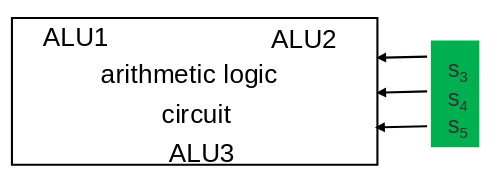
\includegraphics[scale=0.25]{execexample}
			\begin{tabular}{|c|c|c|c|}
				\hline
				$S_3$ & $S_4$ & $S_5$ & $\text{ALU}_3$ \\
				\hline
				0 & 0 & 0 & $\text{ALU}_1 + \text{ALU}_2 + C_{in}$ \\
				\hline
				0 & 0 &1 & $\text{ALU}_1 - \text{ALU}_2 - (\neg C_{in})$ \\
				\hline
				0 & 1 & 0 & $\text{ALU}_2 - \text{ALU}_1 - (\neg C_{in})$ \\
				\hline
				0 & 1 & 1 & $\text{ALU}_1 \lor \text{ALU}_2$ \\
				\hline
				1 & 0 &0 & $\text{ALU}_1 \land \text{ALU}_2$ \\
				\hline
				1 & 0 & 1 & $(\neg \text{ALU}_1) \land \text{ALU}_2$ \\
				\hline
				1 & 1 & 0 & $\text{ALU}_1 \oplus \text{ALU}_2$ \\
				\hline
				1 & 1 &1 & $\text{ALU}_1 \leftrightarrow \text{ALU}_2$ \\
				\hline
			\end{tabular}
		\end{table}
	\end{center}
\end{example}

\paragraph{Status register}
Informs the control unit about the state of the processor after an operation via single bits. Common \textbf{flags} (the bits) are:
\begin{itemize}
	\item \textbf{Auxiliary Carry} (AF): indicates a carry between the \textit{nibbles} (4bit halves of a byte). It's used for \textbf{binary coded digit} arithmetic. \footnote{Also called \textit{half-carry flag}, \textit{digit carry}, \textit{decimal adjust flag}.} 
	\item \textbf{Carry Flag} (CF): indicates a carry produced by the MSBs. Allows for additions and subtractions between \textbf{numbers larger} that a single word through sequential operations that take the carry into account.
	\item \textbf{Zero Flag} (ZF): if the result of an operation was zero. Used for \textbf{conditional branches}.
	\item \textbf{Even Flag} (EF): if the result is \textbf{even} or \textbf{odd} based on the LSB
	\item \textbf{Sign Flag} (SF): if the result is negative (MSB is 1) in two complements. Used for \textbf{conditional branches}.
	\item \textbf{Parity Flag} (PF): if the number of set bits is even or odd. Used for \textbf{error detection}.
	\item \textbf{Overflow Flag} (OF): if the result of an operation is too large to be represented 
\end{itemize}

\paragraph{Program Status Word}
Status register combined with control register determine the current \textbf{state} of a processor. If we combine that with the \textbf{program counter} we get the state of a processor at a certain instruction of a program. It gets:
\begin{itemize}
	\item \textbf{Pushed} to stack before context switch
	\item \textbf{Pulled} from stack to continue execution of an interrupted program
\end{itemize}

\paragraph{Address generation unit}
\begin{wrapfigure}[3]{r}{3.3cm}
	\vspace{-0.5cm}
	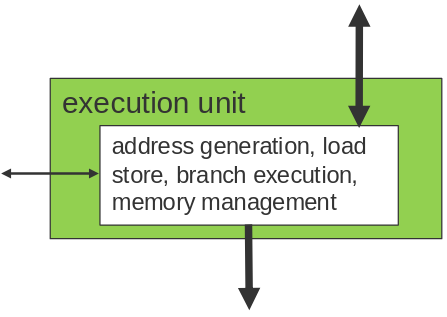
\includegraphics[width=3.3cm]{execunit2}
\end{wrapfigure}
Calculates the address based on control signals from the control unit and possible additional content of the registers.

\subsubsection{Registers}
\begin{wrapfigure}[10]{r}{8cm}
	\vspace{-1cm}
	\begin{center}
		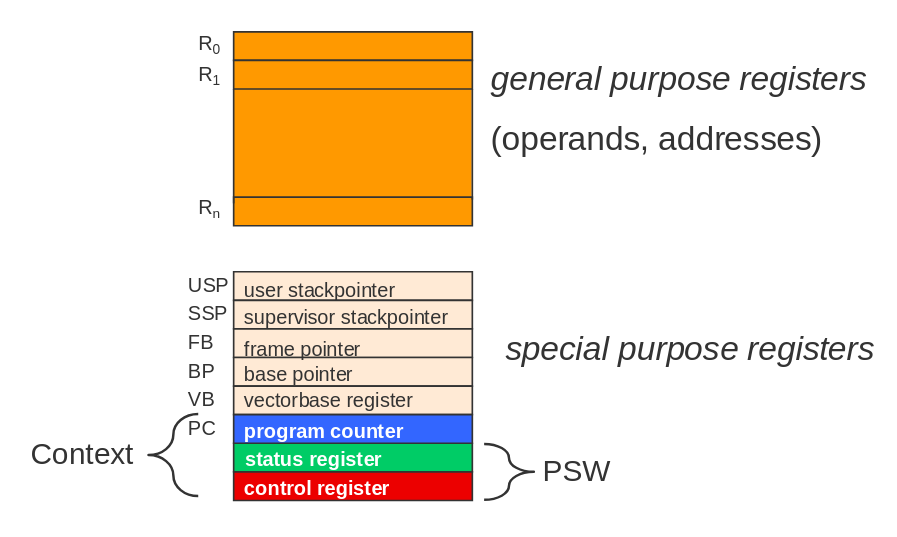
\includegraphics[width=8cm]{registerfile}
	\end{center}
\end{wrapfigure}
They extend the registers of the execution unit, containing frequently used operands. It's a very \textbf{fast} memory with a low access time ($<1\text{ms}$).\\
The \textbf{selection} of single registers happens through dedicated \textbf{control lines} without any address decoding. It can also offer other functions:
\begin{itemize}
	\item \textbf{Increment} and \textbf{decrement}
	\item \textbf{Shift}
	\item Set to \textbf{zero}
\end{itemize}
There are several independent I/O ports, allowing \textbf{simultaneous} writing and reading of different registers. In modern processors up to 4 writes and 8 reads in one clock cycle.

\paragraph{Base pointer}
The base pointer special register contains the start address of a memory region (e.g. an array). The \textbf{index} represents the offset relative to the base pointer. The sum of the two gives the absolute address of an element.

\begin{center}
	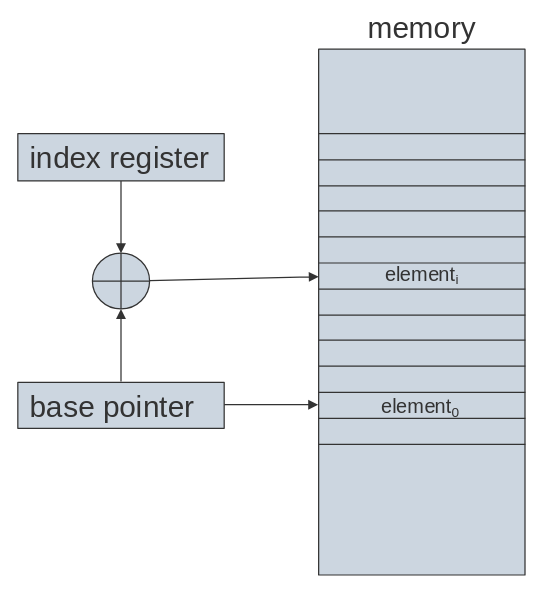
\includegraphics[scale=0.3]{basereg}
\end{center}

\paragraph{Index register}
\noindent The \textbf{index register} has special functions to save time from the ALU:
\begin{itemize}
	\item \textbf{Post-increment}: automatic increment of the register by $n$ after addressing the memory
	\item \textbf{Pre-decrement}: automatic decrement of the register by $n$ before addressing the memory
	\item \textbf{Auto-increment/decrement}
	\item \textbf{Autoscaling} by a factor $n$, used to access memory in bytes or words
\end{itemize}

\paragraph{Stack pointer}
Part of the main memory organized with \textbf{LIFO} principle. It stores the \textbf{PSW} during the subroutine calls/interrupts, allows the passing of the \textbf{parameters} and stores \textbf{temporary results}. Processors usually have different types (e.g. user, system, data).\\
The \textbf{stack pointer} contains the address of the newest data on the stack.\\
Two operations are allowed:
\begin{itemize}
	\item \textbf{PUSH}: transfer the value of a register on top of the stack
	\item \textbf{POP}: load a register with the value on top of the stack and remove it
\end{itemize}

\subsubsection{System Bus Interface}
The Bus Interface Unit is the connection of the microprocessor to all the other components of the computer. The main purposes are:
\begin{itemize}
	\item \textbf{Buffering} of \textit{addresses} and \textit{data} (operand and instructions)
	\item \textbf{Adaptation} of \textit{clock cycle}, \textit{bus width} and \textit{voltages}
	\item \textbf{Tristate}: detaches the processor from the external bus
\end{itemize}
\begin{center}
	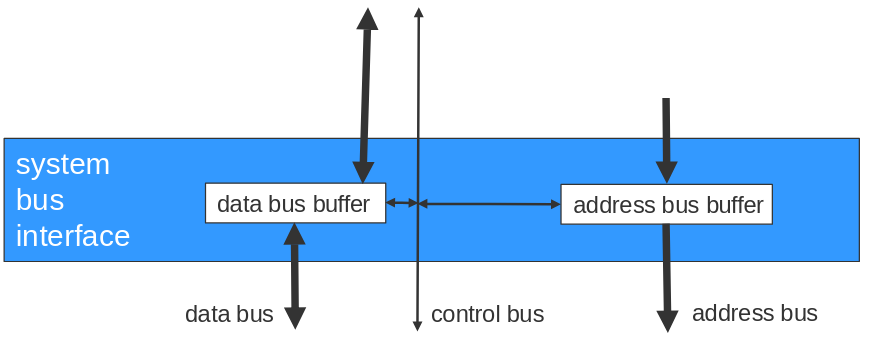
\includegraphics[scale=0.4]{bus}
\end{center}

\subsection{Pipelining}
The performance of a computer can be improved either by improving the \textbf{hardware} using new technologies and materials (expensive and with limitations) or by increasing the \textbf{parallelism} (more transistors, wider bus, replicated function units).

\subsubsection{Structural enhancements}
The classification of computer architectures, according to Flynn, is composed of four types.
\paragraph{SISD} Single Instruction Single Data consists in one single stream of instructions that operate on the data (classic Von Neumann).

\paragraph{SIMD} Single Instruction Multiple Data is where all processors perform the same instruction on different data (array processor). E.g. image processing, where each processor handle one part of the image.

\paragraph{MIMD} Multiple Instruction Multiple Data where all processors perform different instructions on different data. The one it's mostly used today.

\paragraph{MISD} Multiple Instruction Single Data where several instructions operate on a single data. Not very common but could be use e.g. for fault tolerance (and then compare the results).

\begin{figure}[!h]
	\hfill
	\subfigure[SISD]{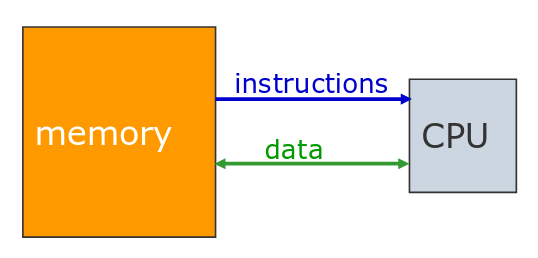
\includegraphics[scale=0.2]{sisd}}
	\hfill
	\subfigure[SIMD]{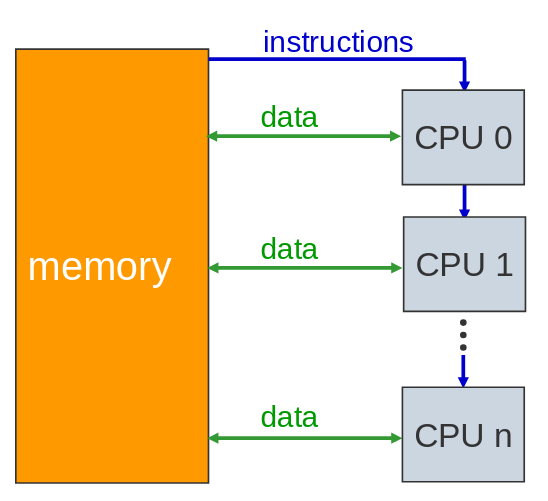
\includegraphics[scale=0.2]{simd}}
	\hfill
	\subfigure[MIMD]{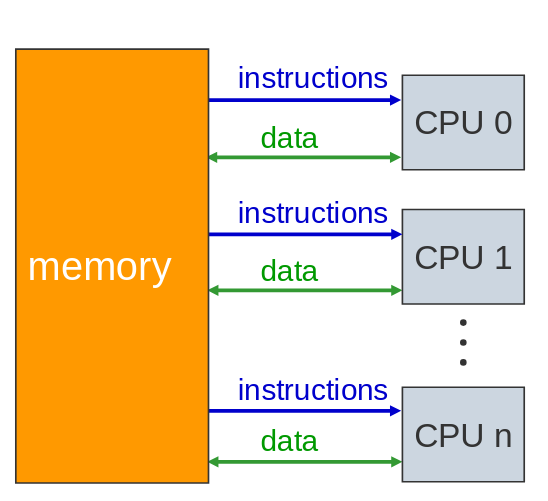
\includegraphics[scale=0.2]{mimd}}
	\hfill
\end{figure}

\subsubsection{Pipeline processing}
Pipelining is the \textbf{subdivision} of an operation into several phases or sub operations and their \textbf{synchronous execution} in different functional unit (each one responsible for its own).\\
Each stage is a pipeline \textbf{stage} or \textbf{segment}. The whole pipeline is clocked in a way that each cycle instruction can be shifted one step further through it.\\
Ideally we have a $\mathbf{k}$ \textbf{stage pipeline} with $k$ cycles and $k$ stages, allowing $k$ instructions to be executed at the same time and needing $k$ cycles to complete.

\begin{definition}[Latency]
	Duration of the complete processing of an instruction. The time an instruction needs to go through	all $k$ stages of the pipeline.
\end{definition}

\begin{definition}[Throughput]
	Number of instructions leaving the pipeline per clock cycle. It should be close to $1$ for a \textbf{scalar} processor and may be $> 1$ for \textbf{superscalar} processors.
\end{definition}

\paragraph{Speedup}
A \textbf{standard} processor without pipeline, considering $n$ instructions and $k$ stages, needs:
\begin{equation}
	n \cdot k \text{ cycles}
\end{equation}
A \textbf{pipelined} processor needs, assuming $k$ cycles latency and throughput $=1$, needs:
\begin{equation}
	k + (n-1) \text{ cycles}
\end{equation}
Assuming an infinite number of instructions the \textbf{speed up} of a processor with a $k$ staged pipeline is:
\begin{equation}
	\lim_{n \to \infty} \frac{n \cdot k}{k+n-1} = \lim_{n \to \infty} \frac{k}{\frac{k}{n}+1-\frac{1}{n}} = \frac{k}{0+1-0} = k
\end{equation}

\paragraph{Five stage pipeline}
It consists in these five stages:
\begin{enumerate}
	\item \textbf{Instruction Fetch} (IF): load the instruction from memory or cache into the opcode register and increment the program counter
	\item \textbf{Instruction Decode} (ID): generate internal signals based on the opcode or jump to the appropriate microprogram
	\item \textbf{Operand Fetch} (OF): load the operands from the registers into the operand registers of the ALU and calculate the effective address for load/store or branch instructions
	\item \textbf{Execution} (EXE)
	\item \textbf{Write Back} (WB): write the result into a register or memory if needed. Load/store instructions put the address on the address bus and transfer the data to the memory
\end{enumerate}
\begin{center}
	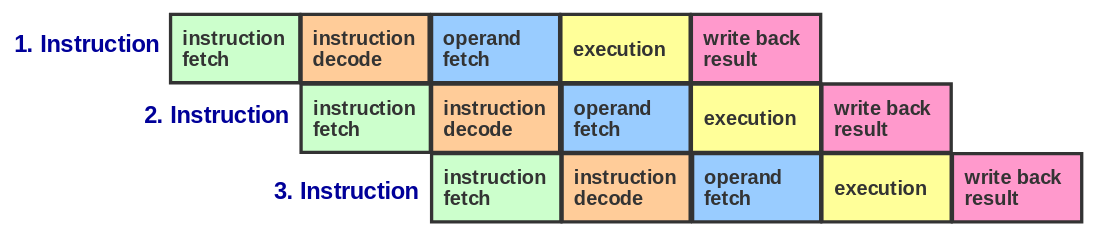
\includegraphics[scale=0.3]{pipeline}
\end{center}

\paragraph{Two instruction}
If we assume that:
\begin{itemize}
	\item Instruction Fetch requires half the time of all other stages
	\item We can have arbitrary many other functional units
\end{itemize}
then we can have an improved pipeline that works in parallel:
\begin{center}
	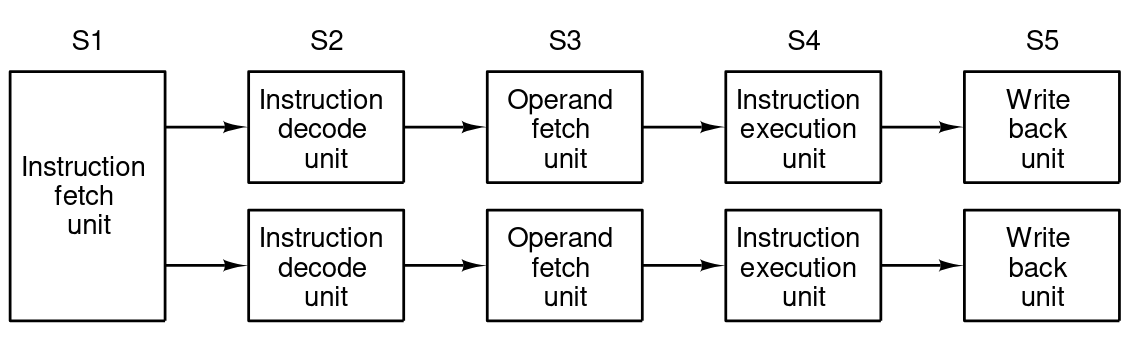
\includegraphics[scale=0.2]{2pip}
\end{center}

\paragraph{Specialized execution units}
\begin{center}
	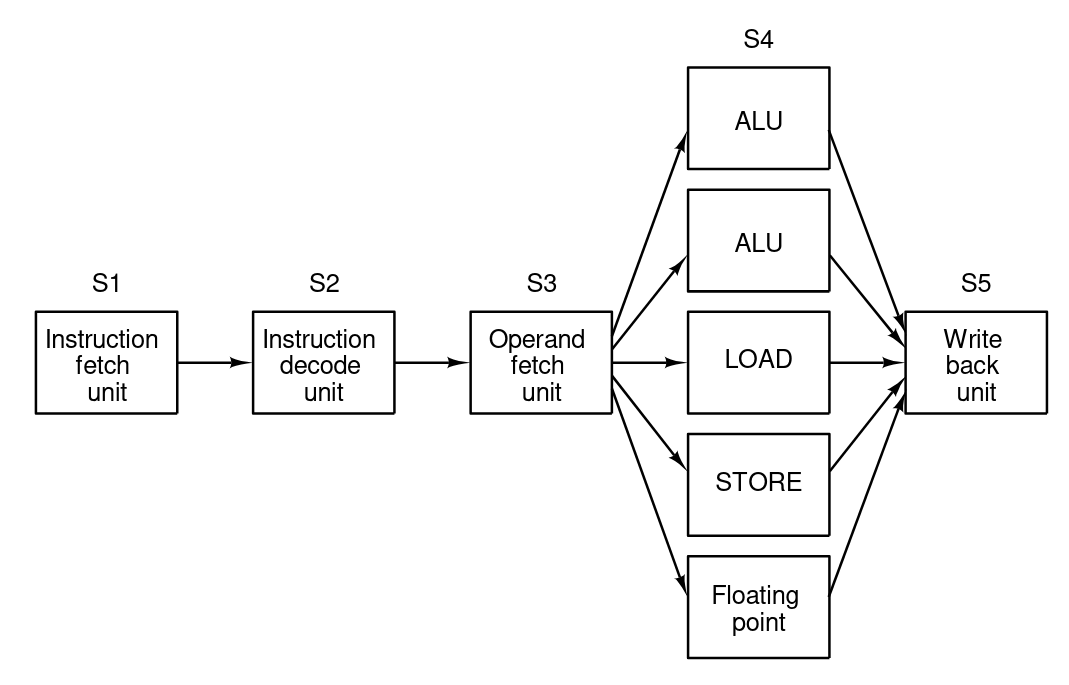
\includegraphics[scale=0.3]{specexe}
\end{center}

\paragraph{MIPS pipeline}
The MIPS pipeline is defined as follows:
\begin{enumerate}
	\item \textbf{Instruction Fetch} (IF): fetch instruction from \textit{main} memory
	\item \textbf{Instruction Decode} (ID): read operand registers while decoding the instruction (simultaneous thanks to format of MIPS instructions)
	\item \textbf{Execution} (EXE): \textbf{execute} the operation (arithmetical and logical operations) or \textbf{calculate} an address (\textit{load} and \textit{store})
	\item \textbf{Memory Access} (MEM): access an operand in data memory\footnote{If the instruction is \textit{load} or \textit{store}, otherwise nothing happens.}
	\item \textbf{Write Back} (WB): write the result into a register
\end{enumerate}
With this pipeline the affected registers are \textbf{written} into during the first half of the WB stage while the operand registers are \textbf{read} during the second half of the ID stage.

\begin{center}
	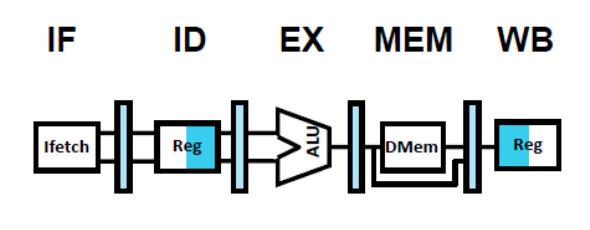
\includegraphics[scale=0.4]{mips}
\end{center}

\subsubsection{Pipeline hazards}
\begin{definition}[Pipeline hazard]
	Phenomena that may disrupt the smooth execution of a pipeline.
\end{definition}

\begin{example}
	If we assume a unified cache with a single read port (instead of separate instruction and data caches), a memory read conflict appears among IF and OF stages. The pipeline has to stall (\textbf{pipeline bubble}) one of the accesses until the required memory port is available.
\end{example}

\hfill

\paragraph{Data hazard} These type of hazards happen when there are \textbf{dependencies} between instructions, causing an overlapping between their execution. There are three types:
\begin{itemize}
	\item \textbf{Read After Write} (RAW): instruction 2 tries to read the register before instruction 1 writes it
	\item \textbf{Write After Read} (WAR): instruction 2 tries to write a register before instruction 1 reads it
	\item \textbf{Write After Write} (WAW): instruction 2 writes a register before instruction 1 writes it
\end{itemize}

\begin{example}[RAW in MIPE pipeline]
	Let's consider this piece of code:
	\begin{lstlisting}[language={[x86masm]Assembler}]
		mov R1, A
		mov R2, B
		add R2, R1, R2
		mul R1, R2, R1
	\end{lstlisting}
	We will have the following dependencies:
	\begin{center}
		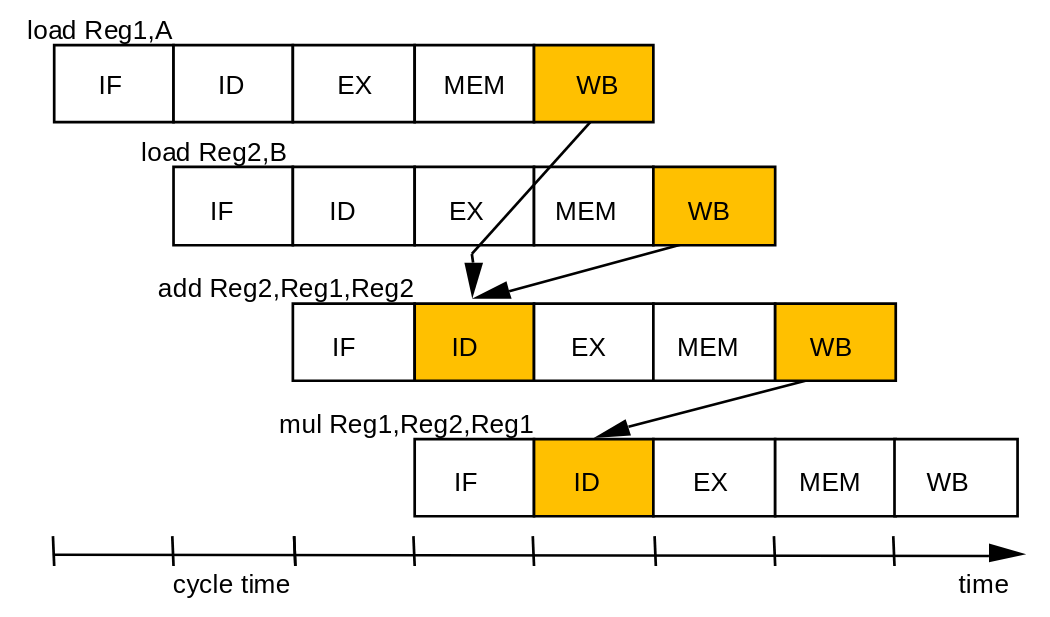
\includegraphics[scale=0.3]{rawex}
	\end{center}
\end{example}

\begin{observation}[WAR and WAW]
	In a five stage pipeline WAR and WAW can't happen since all instructions take five stages and the reads are always in stage 2 while the writes in stage 5.
\end{observation}

\subparagraph{Software solutions}
Software solutions involve two options:
\begin{itemize}[leftmargin=+1.5cm]
	\item Put \textbf{no-op} operations after each instruction that may cause a hazard
	\item \textbf{Reorder} the instructions
\end{itemize}

\subparagraph{Hardware solutions}
Hardware solutions require a hazard detection logic:
\begin{itemize}[leftmargin=+1.5cm]
	\item \textbf{Stalling} or \textbf{interlocking}: we stall the pipeline for one or more cycles
	\item \textbf{Forwarding}: we forward either the \textbf{result} or the \textbf{load}ed data directly to the next stage where it's needed. It may be necessary to also use \textbf{stalling} since even if forwarded the data may still not be available.
\end{itemize}

\newpage
\begin{example}[Forwarding]
	Let's consider this piece of code:
	\begin{lstlisting}[language={[x86masm]Assembler}]
		add R1, R2, R3
		sub R4, R1, R3
		and R6, R1, R7
		or R8, R1, R9
	\end{lstlisting}
	We will have the following forwarding of both, result and load
	\begin{center}
		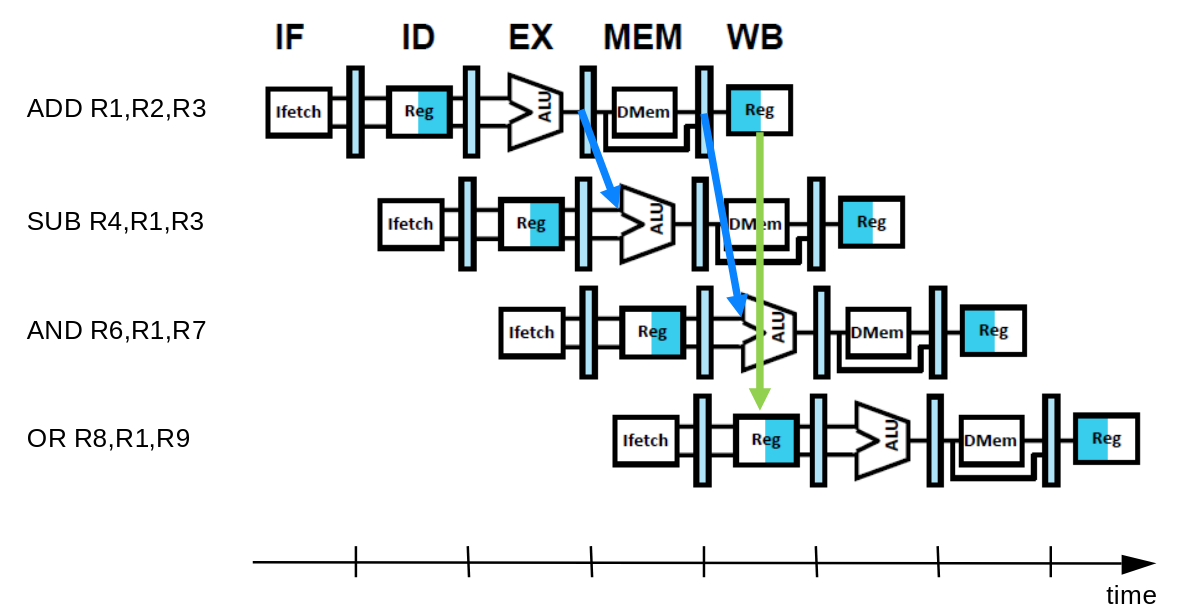
\includegraphics[scale=0.3]{fwex}
	\end{center}
\end{example}

This is how a hardware (\textbf{bypass}) solution can be implemented:
\begin{center}
	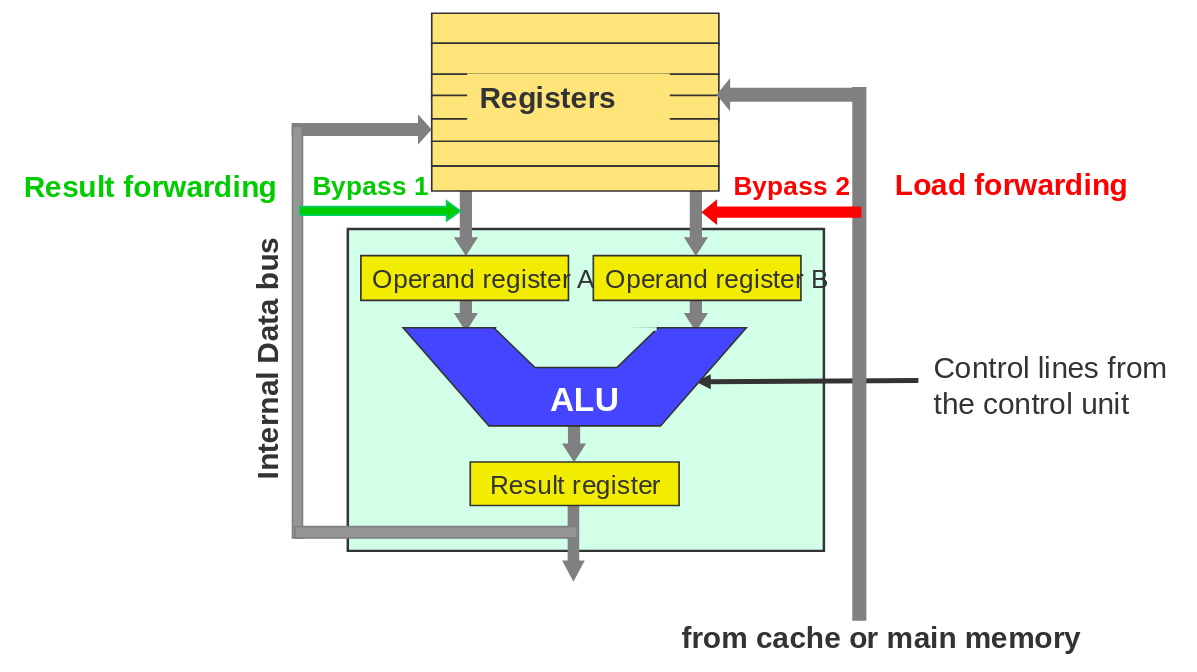
\includegraphics[scale=0.4]{byp}
\end{center}
\newpage

\paragraph{Structural hazard}
Structural hazards may arise from some combinations of instructions that cannot be accommodated because of \textbf{resource conflicts}.
\begin{example}
	If the processor has only one register port and two instructions want to write into it at the same time.
\end{example}

The main solutions are:
\begin{itemize}
	\item \textbf{Arbitration with interlocking}: hardware that performs resource conflict arbitration and interlocks one of the competing instructions
	\item \textbf{Resource replication}: e.g. more write ports. This could arise more dependencies.
\end{itemize}

\paragraph{Control hazard}
Control hazards arise from \textbf{control flow instructions} (e.g. branch, jump).
\begin{example}
	Considering this code:
	\begin{lstlisting}[language={[x86masm]Assembler}]
						cmp R1,R2
						adc R4,R5,R4
						beq Label
						add R3,R1,R2
		Label: 		sub R6,R4,R5
						sll R0
	\end{lstlisting}
	The \textit{add} instruction is still in the pipeline when the jump is executed and therefore it is also executed before it.
	
	\subparagraph{Software solution}
	There are two options:
	\begin{itemize}[leftmargin=+1.5cm]
		\item Put \textbf{no-op} operations after every branch
		\item \textbf{Reorder} the instructions so that the ones that will not affect the branch will be executed right before it
	\end{itemize}
	\subparagraph{Hardware solution}
	There are three options:
	\begin{itemize}[leftmargin=+1.5cm]
		\item \textbf{Interlocking}: the hardware detects the branch and applies the interlocking to stall the next instructions
		\item \textbf{Flushing}: empty the pipeline before releasing the jump
		\item \textbf{Speculative branch}: in case of a \textbf{conditional jump} estimate the result and load the pipeline. If the estimate was wrong, \textit{flush}.
	\end{itemize}
\end{example}

\subsubsection{Branch prediction}
Branch prediction foretells the outcome of conditional branch instructions. IF stage finds a branch instruction and predicts its direction. The branch delay slots are speculatively filled with instruction, either those of:
\begin{itemize}
	\item the consecutively \textbf{following path},
	\item the path at the \textbf{target address}
\end{itemize}
After resolving of the branch direction decide upon correctness of prediction. In case of misprediction discard wrongly fetched instructions. Re-rolling in this case is \textbf{expensive}.

\paragraph{Branch Target Buffer}
The Branch Target Buffer (BTB) or Branch-Target Address Cache (BTAC) stores branch and jump target
addresses. The BTB is accessed during the IF stage and consists of a table with \textbf{branch addresses}, the corresponding \textbf{target addresses}, and \textbf{prediction information}.
There are some variations:
\begin{itemize}
	\item \textbf{Branch Target Cache} (BTC): stores one or more target instructions additionally
	\item \textbf{Return Address Stack} (RAS): a small stack of return addresses for procedure calls and returns is used additional to and independent of a BTB.
\end{itemize}

\paragraph{Static}
The prediction for an individual branch	does not change and comprises of:
\begin{itemize}
	\item \textbf{machine-fixed}: the prediction can be \textbf{wired} into the processor by predicting that all branches will be taken (backwards) or all not taken (forward)
	\item \textbf{compiler-based}: opcode in branch instructions allows the compiler to set it. Then it can either \textbf{examine} the program code or use \textbf{profile information} from earlier runs
\end{itemize}
\paragraph{Dynamic}
In dynamic branch prediction the prediction is decided on the \textbf{computation history} of the program execution. In general gives better results than static but at the cost of \textbf{increased hardware complexity}.
\subparagraph{Predictors}
A \textbf{one-bit} predictor correctly predicts a branch at the end of a loop iteration, as long as the loop does not exit. In nested loops, a one-bit prediction scheme will cause two mispredictions for the inner loop:
\begin{itemize}
	\item One at the \textbf{end} of the loop, when the iteration exits the loop instead of looping again
	\item One when executing the \textbf{first loop iteration}, when it predicts exit instead of looping
\end{itemize}
This is avoided by a \textbf{two-bit} predictor scheme, where a prediction must miss twice before it is changed when a two-bit prediction scheme is applied.
\begin{figure}[!h]
	\centering
	\subfigure[one-bit]{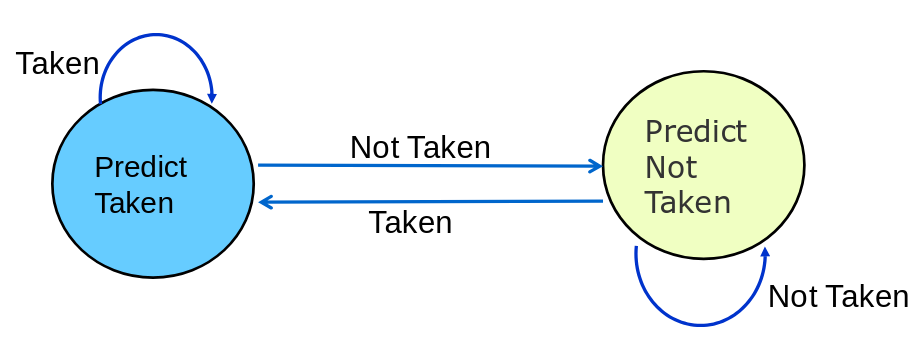
\includegraphics[scale=0.23]{onebit}}
	\hfill\\
	\subfigure[two-bit Hysteresis scheme]{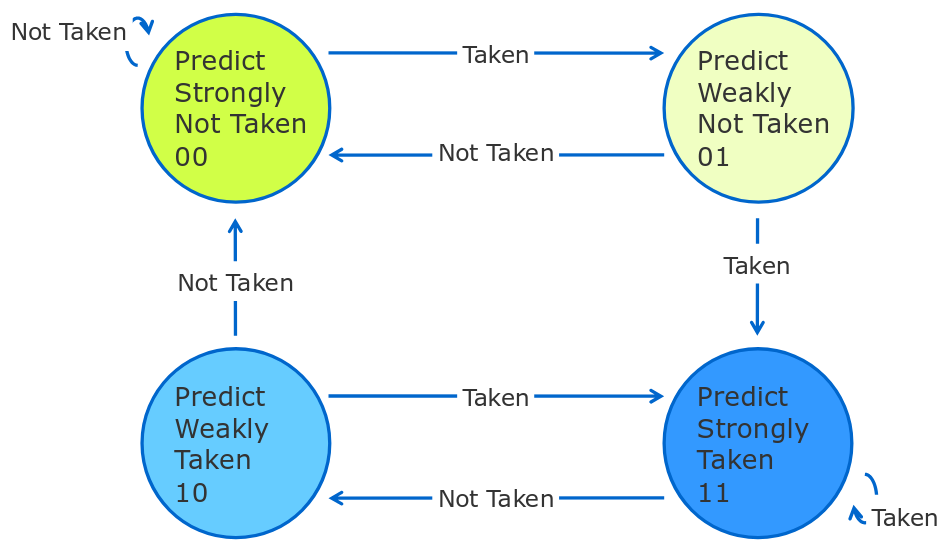
\includegraphics[scale=0.23]{twobit}}
	\hfill
	\subfigure[two-bit 	Saturation Counter scheme]{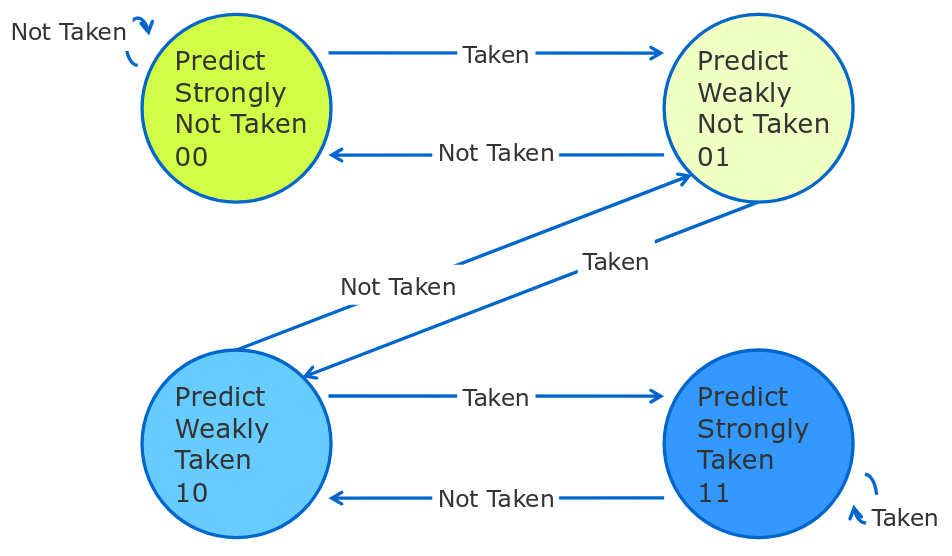
\includegraphics[scale=0.23]{twobitsat}}
	\hfill
\end{figure}

\begin{center}
	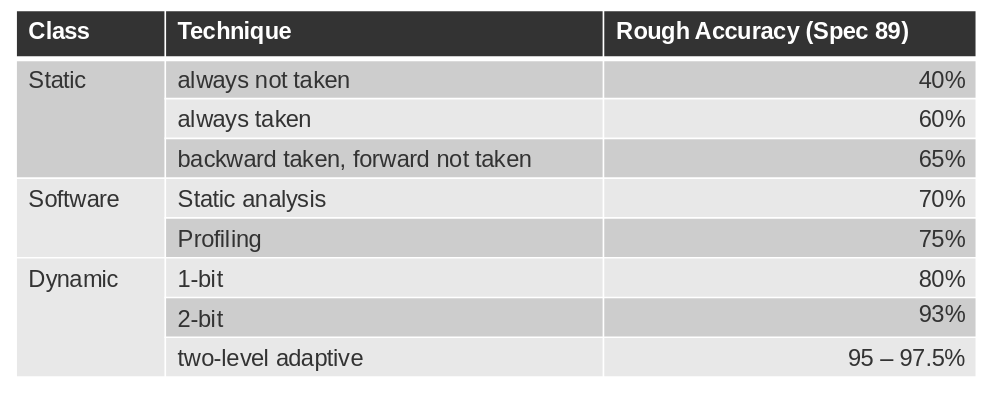
\includegraphics[scale=0.3]{predstat}
	\captionof{figure}{Statistics about different techniques}
\end{center}

\paragraph{Predicate instructions}
It provides \textbf{predicated} or \textbf{conditional instructions} and \textbf{predicate registers}, which are used as an additional input operand. They are able to remove a branch and keep the pipeline busy but it complicates the instruction set and consume resources.

\subsection{Superscalar processors}
\begin{definition}
	Superscalar machines are distinguished by their ability to dynamically issue multiple instructions each clock cycle from a conventional linear instruction stream.
\end{definition}

\begin{center}
	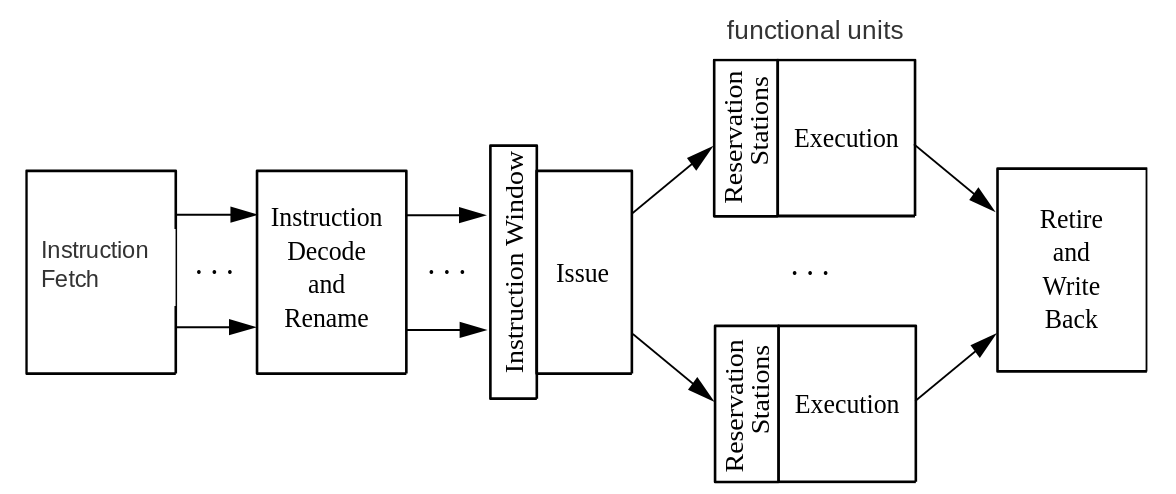
\includegraphics[scale=0.35]{super}
\end{center}

A superscalar pipeline is divided in three sections:
\begin{itemize}
	\item \textbf{in-order}
	\begin{itemize}
		\item \textit{fetch}: get the commands
		\item \textit{decode}: decode the new instructions
		\item \textit{rename}: externally visible register are mapped to internal shadow registers, stored in a rename map (e.g. \textit{alias table}), so that core execution units are free from name dependencies
		\item \textit{issue} if \textit{in-order} issue processor. The waiting instructions in the \textbf{waiting window} are examined and then simultaneously (up to the \textit{issue bandwidth}) \textbf{issued} to the \textbf{functional units}
	\end{itemize}
	\item \textbf{out-of-order}
	\begin{itemize}
		\item \textit{issue} if out-of-order issue processor
		\item \textit{execution}: there is a \textbf{reservation station}, a buffer that contains a single instruction operands. There may be one for multiple units. When all the operands are ready the instruction is \textbf{dispatched}.
		\item \textit{completion}: when the result is ready for forwarding and buffering. The reservation station gets freed and the state of the execution (can be an interrupt) is noted in the \textbf{reorder buffer}
		\item \textit{Commitment}: after completion an instruction gets committed if:
		\begin{itemize}
			\item al previous instructions are committed or can be committed in the same cycle
			\item if no interrupt occurred before and during the execution
			\item if the instruction is not speculative anymore
		\end{itemize}
	\end{itemize}
	\item \textbf{in-order}
	\begin{itemize}
		\item \textit{retirement}: an instruction retires when the reorder buffer is freed either because of a commit or a delete
		\item \textit{write-back}: the result of the instruction is made permanent in the architectural register
	\end{itemize}
\end{itemize}
% !TeX spellcheck = en_US
\newpage
\section{Instruction set architecture}
The ISA level is the classical boundary between SW and HW and defines what is visible or not to the user. High level languages are translated into instructions from the ISA.

\subsection{CISC}
Complex Instruction Set Computer exist for chips, high programming languages and special purpose applications that favor complex instructions.\\
The \textbf{positive sides} are:
\begin{itemize}
	\item Execution of a single complex instruction is \textbf{faster} than the execution of a microprogram that does the same thing
	\item Shorter programs, thus \textbf{faster loading times}
	\item Direct \textbf{support of programming constructs} from higher programming languages
	\item Support of specialized \textbf{powerful compilers}
	\item \textbf{Compatibility}
	\item Support of \textbf{special purpose applications} (e.g. matrix operations)
\end{itemize}
The \textbf{negative sides}:
\begin{itemize}
	\item Needs faster main memories and the use of cache memory speed-up program execution
	\item Complex instructions can sometimes be \textbf{replaced with} several \textbf{simpler} and faster ones
	\item \textbf{Long development} cycle of CPUs
	\item \textbf{Complex control units}
	\item Large microprograms with potentially \textbf{more errors}
	\item Real programs often use only a small portion of the instructions
\end{itemize}

While there are many powerful instructions, usually just $20\%$ of them are used, still maintaining the complex format. Furthermore, many classical CISC architectures have a $\text{CPI}>2$.\\
That being said, optimized code for Pentium, Itanium and others usually have a $\text{CPI} \approx1$.

\subsection{RISC}
Reduced Instruction Set Computer consists of:
\begin{itemize}
	\item Few \textbf{instructions} ($\leq 128$)
	\item $\leq 4$ \textbf{instruction formats}
	\item Fixed \textbf{instruction length} of $32$ bit
	\item $\leq 4$ \textbf{addressing modes}
\end{itemize}
If possible all instructions should be implemented so that they can finish in a single cycle. As a consequence, there is no micro programming in RISC.

\begin{note}
	Early RISC processors had SW controlled pipeline (NOPs) instead of special hardware.
\end{note}
\subsubsection{Memory access}
This instruction set uses the \textbf{register/register} or \textbf{load/store} principle: \textbf{memory access} is possible only via \textit{load} and \textit{store} operations, while all other operations are done on registers.

\subsubsection{Pros and cons}
The \textbf{positive sides} are:
\begin{itemize}
	\item Single chip implementation, allowing the use of the saved \textbf{space} for something else
	\item Short development cycle
	\item \textbf{Higher clock rates}, \textbf{pipelines}
\end{itemize}
The main \textbf{downside} is the bottleneck in the memory interface, since main memory is much slower than internal registers and cache.

\subsection{Addressing modes}
There are different possibilities to calculate the address of an operand or the branch target address in the memory.
\subsubsection{Static}
The \textbf{classical} way is through an \textbf{absolute} address. This means that the location is determined at compilation and accessing dynamic structures requires a change in the address for each instruction.
\subsubsection{Dynamic}
In this case the calculation of the address is done at runtime: the instruction triggers the calculation of the \textbf{logical address} and then the memory management unit finds the physical one.
\begin{center}
	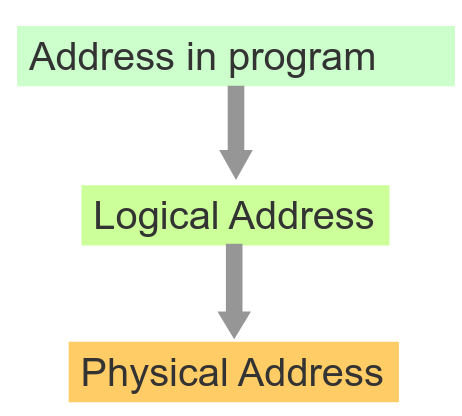
\includegraphics[scale=0.3]{dac}
\end{center}

\newpage
\subsection{Non linear execution}
Usually a program follows a non linear execution due to many reasons:
\begin{itemize}
	\item Jumps, branches
	\item Procedure calls, subroutines, method calls
	\item Multi-threading, parallel processing, co-routines
	\item Hardware interrupts
	\item Traps, software interrupts
\end{itemize}

\begin{figure}[!h]
	\centering
	\subfigure{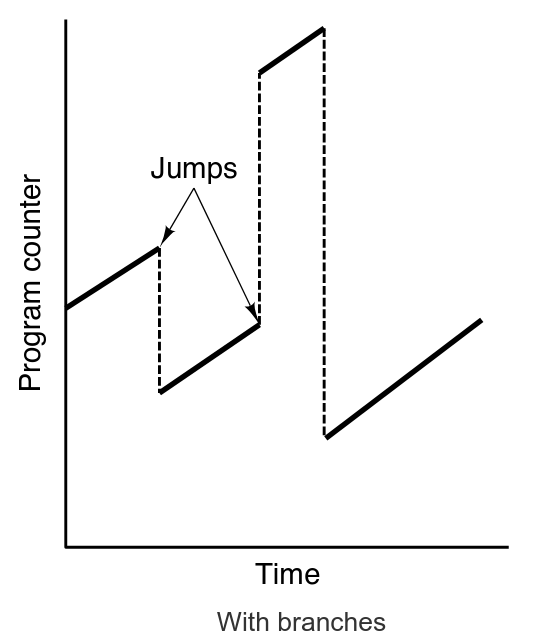
\includegraphics[scale=0.23]{branch}}
	\hfill
	\subfigure{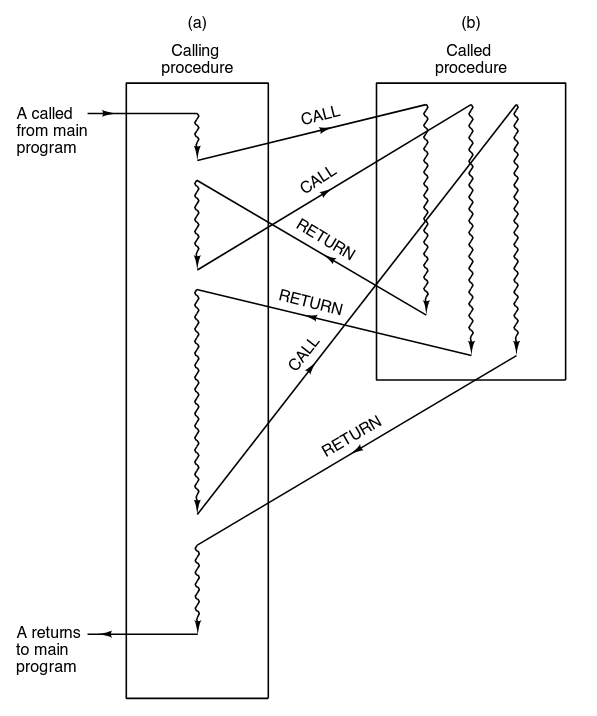
\includegraphics[scale=0.23]{procall}}
	\hfill
	\subfigure{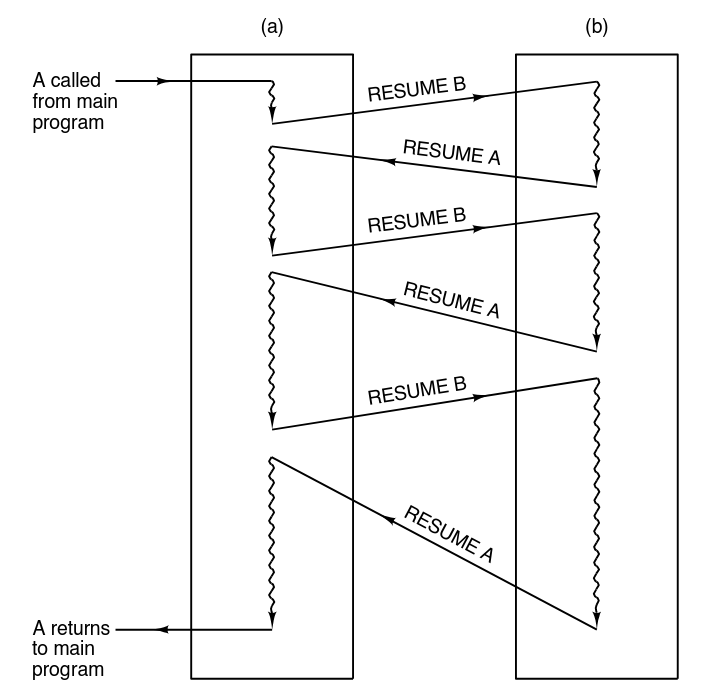
\includegraphics[scale=0.23]{corout}}
	\hfill
\end{figure}

\begin{definition}[Exception]
	Interruption of the programmed control flow of instructions during runtime.
\end{definition}
\subsubsection{Causes}
Exceptions may be caused by:
\begin{itemize}
	\item \textbf{External} reasons: asynchronous events such as
	\begin{itemize}
		\item \textit{RESET}: reset of the processor (e.g. power button)
		\item \textit{HALT}: stop the execution of the processor (e.g. to avoid conflict on memory access)
		\item \textit{ERROR}: call of an error routine (e.g. bus errors)
		\item \textbf{Interrupts}: request triggered by an external device (e.g. to announce incoming data). They can be \textit{maskable} or \textit{non maskable}
	\end{itemize}
	\item \textbf{Internal} reasons: synchronous events such as
	\begin{itemize}
		\item \textbf{Software interrupts}: \textit{INT} instructions in the program triggers an interrupt (e.g. system call)
		\item \textbf{Traps}: exception caused by internal events (e.g. overflow)
	\end{itemize}
\end{itemize}
\newpage
\subsubsection{Handling}
Handling of exceptions requires specialized routines called \textbf{Interrupt Service Routine} (ISR). They have the same structure as a subprogram but with some differences:
\begin{table}[!h]
	\centering
	\begin{tabular}{|p{2cm}|p{3cm}|p{3.5cm}|}
		\hline
		\textbf{Activity} & \textbf{Subprogram} & \textbf{ISR} \\
		\hline
		\textit{Activation} & \textit{call} subroutine & \textit{INT} instruction or hardware activation\\
		\hline
		\textit{Return after completion} & \textit{RET} instruction & \textit{RETI} instruction \\
		\hline
		\textit{Calculation of starting address} & Written in calling program & Determined via interrupt table \\
		\hline
		\textit{Saving status} & Typically saves PC on a stack & Saves PC and PSW on a stack\\
		\hline
	\end{tabular}
\end{table}

\noindent The \textbf{steps} of an ISR are:
\begin{enumerate}
	\item Interrupt activation
	\item Finalize the current instruction
	\item Check if SW or internal/external HW
	\item Check if \textit{Interrupt Enable} bit is set
	\item If HW, find the source and activate the acknowledge (INTA)
	\item Reset \textit{Interrupt Enable} to avoid additional interrupts
	\item Save PSW and PC on stack
	\item Calculate the start address and load it to PC. Usually done through the \textbf{Interrupt Vector Table}, which is at a specific location and contains the start addresses of the ISRs
	\begin{center}
		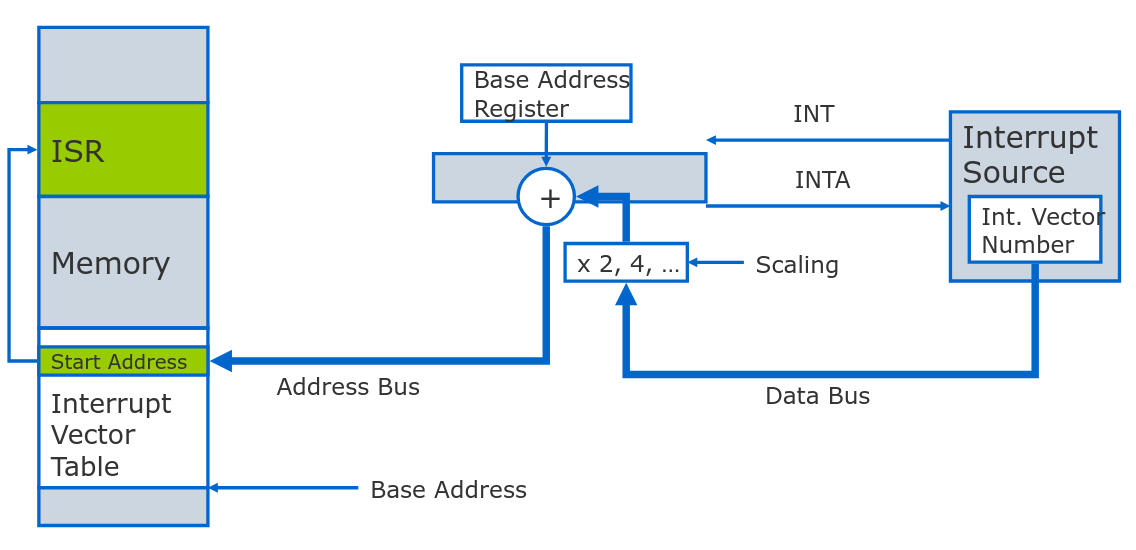
\includegraphics[scale=0.3]{isr}
	\end{center}
	\item Execute the ISR:
	\begin{itemize}
		\item Push the used register on stack
		\item Set the interrupt bit to allow more interrupts
		\item Execute ISR
		\item Pop the registers from stack
		\item Return using \textit{IRET}
	\end{itemize}
	\item Restore PSW and PC and continue the original program
\end{enumerate}

\subsubsection{Multiple interrupts}
During the handling of an interrupt, more may happen. There are two different approaches to handle them:
\begin{itemize}
	\item \textbf{Fair}: continue cyclic polling following the last served source, granting an equal chance of being served
	\begin{center}
		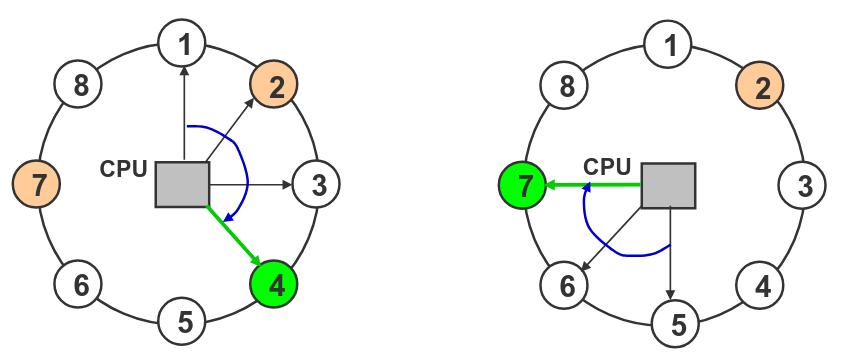
\includegraphics[scale=0.3]{fair}
	\end{center}
	\item \textbf{Priority}: cyclic polling always starts at a predetermined sourced. Every source gets a different priority and the higher one are served first.
	\begin{center}
		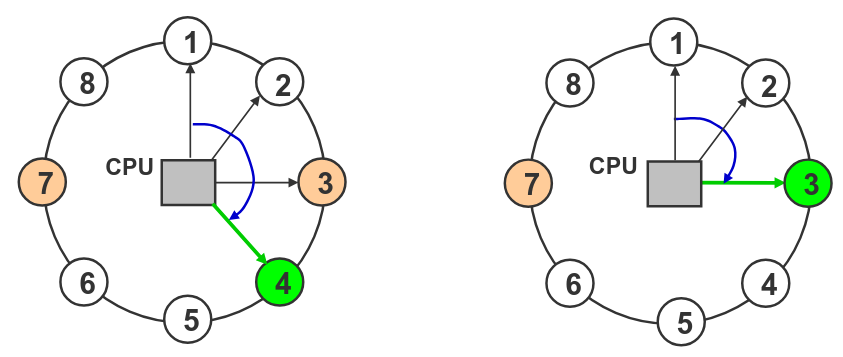
\includegraphics[scale=0.3]{priority}
	\end{center}
\end{itemize}
It's possible to use \textbf{hardware daisy chaining} to handle multiple interrupts, using specialized hardware for prioritization and identification of interrupts. Each source for an interrupt uses dedicated HW for connecting with a successor and a predecessor. The first one has the highest priority.
\begin{center}
	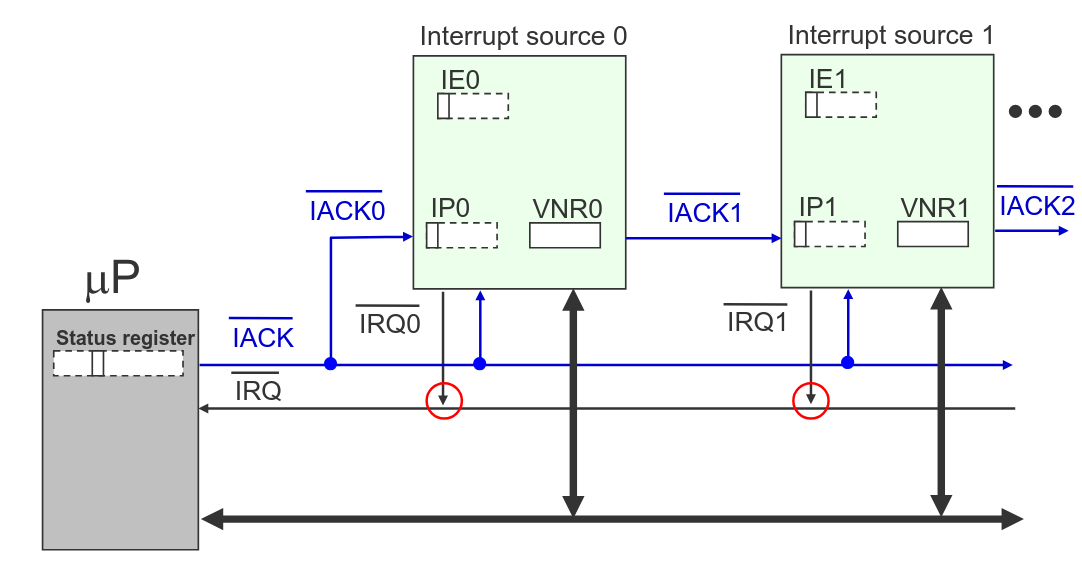
\includegraphics[scale=0.3]{daisychain}
\end{center}
\end{document}
